\documentclass{article}

\usepackage[spanish, english]{babel}

\usepackage[letterpaper,top=2cm,bottom=2cm,left=3cm,right=3cm,marginparwidth=1.75cm]{geometry}

\usepackage{graphicx}
\usepackage[colorlinks=true, allcolors=blue]{hyperref}
\usepackage[strict]{changepage}
\usepackage{amsmath,amsthm,amssymb,amsfonts, color, comment, graphicx, environ}
\usepackage{xcolor}
\usepackage{listings}
\usepackage{tcolorbox}
\usepackage{mdframed}
\usepackage{tikz}
\usepackage{tkz-fct}
\usetikzlibrary{calc,arrows,babel,shapes,spy,positioning,snakes}
\usepackage{mathtools}
\usepackage{physics}
\usepackage{calligra}
\usepackage{csquotes}
\usepackage{tensor}
\usepackage[thicklines]{cancel}
\usepackage{pstricks}
\usepackage{fancyhdr}
\usepackage{multicol}
\usepackage{float}
\usepackage[shortlabels]{enumitem}
\usepackage{indentfirst}
\usepackage{hyperref}
\hypersetup{
	colorlinks=true,
	linkcolor=blue,
	filecolor=magenta,      
	urlcolor=blue,
}
\usepackage[T1]{fontenc}
\usepackage{titlesec}

%%%%%%%%%%%%%%%%%%%% Colores %%%%%%%%%%%%%%%%%%%%

%%%%% COLORES PASTEL %%%%%
\definecolor{moradopastel}{RGB}{213,201,255}
\definecolor{rosapastel}{RGB}{254,202,202}
\definecolor{azulpastel}{RGB}{217,238,251}
\definecolor{verdepastel}{RGB}{204,252,220}
\definecolor{rojopastel}{RGB}{255,109,109}
%%%%% COLORES PASTEL %%%%%

%%%%% GRISES %%%%%
\definecolor{grisclaro}{RGB}{247, 249, 249}
\definecolor{grisclaro2}{RGB}{240, 243, 244}
\definecolor{gris}{RGB}{191, 201, 202}
%%%%% GRISES %%%%%

%%%%% HTML page %%%%%
\definecolor{IndianRed}{RGB}{205, 92, 92}
\definecolor{LightCoral}{RGB}{240, 128, 128}
\definecolor{Salmon}{RGB}{250, 128, 114}
\definecolor{DarkSalmon}{RGB}{233, 150, 122}
\definecolor{LightSalmon}{RGB}{255, 160, 122}
%%%%% HTML page %%%%%

%%%%% MIS COLORES %%%%%
\definecolor{Rojop}{RGB}{203, 67, 53}
\definecolor{Azulp}{RGB}{41, 128, 185}
\definecolor{Verdep}{RGB}{20, 120, 100}
\definecolor{Amarillop}{RGB}{255, 187,0}
\definecolor{Naranjap}{RGB}{230, 126, 34}
\definecolor{Moradop}{RGB}{108, 99, 255}
\definecolor{Blancop}{RGB}{254, 254, 254}
\definecolor{Negrop}{RGB}{0,0,0}
\definecolor{Cyanp}{RGB}{118, 215, 196}
\definecolor{Olivop}{RGB}{20, 90, 50}
%%%%% MIS COLORES %%%%%

%%%%%%%%%% CODING COLORS %%%%%%%%%%
\definecolor{backgroundcolorgray}{RGB}{61,61,61}
\definecolor{codeYellow}{RGB}{255,216,61}
\definecolor{codeWhite}{RGB}{235,235,235}
\definecolor{codePink}{RGB}{255,0,235}
\definecolor{codeCyan}{RGB}{0,255,255}
\definecolor{codeRed}{RGB}{255,0,55}
%%%%%%%%%% CODING COLORS %%%%%%%%%%
%%%%%%%%%% BASH COLORS %%%%%%%%%%
\definecolor{BASHbackgroundcolor}{RGB}{99,0,39}
\definecolor{BASHgreen}{RGB}{0,140,10}
\definecolor{BASHwhite}{RGB}{245,245,245}
\definecolor{BASHblue}{RGB}{0,125,255}
\definecolor{BASHyellow}{RGB}{255,245,0}
\definecolor{BASHred}{RGB}{200,40,40}
%%%%%%%%%% BASH COLORS %%%%%%%%%%

%%%%%%%%%%%%%%%%%%%% Colores %%%%%%%%%%%%%%%%%%%%

%%%%%%%%%%%%%%%%%%%% Comandos renovados %%%%%%%%%%%%%%%%%%%%

\renewcommand{\qed}{\quad\qedsymbol}
\renewcommand{\qed}{\quad\qedsymbol}
\renewcommand{\theenumi}{\alph{enumi})}

%%%%%%%%%%%%%%%%%%%% Comandos renovados %%%%%%%%%%%%%%%%%%%%

%%%%%%%%%%%%%%%%%%%% Nuevos comandos %%%%%%%%%%%%%%%%%%%%
\newcommand{\scriptr}{\mathcalligra{r}\,}
\newcommand{\boldscriptr}{\pmb{\mathcalligra{r}}\,}
\newcommand{\ie}{\emph{i.e.}} %id est
\newcommand{\eg}{\emph{e.g.}} %exempli gratia
\newcommand{\rtd}[1]{\ensuremath{\left\lfloor #1 \right\rfloor}}
\newcommand{\dirac}[1]{\ensuremath{\delta \left( #1 \right)}}
\newcommand{\diract}[1]{\ensuremath{\delta^3 \left( #1 \right)}}
\newcommand{\e}{\ensuremath{\epsilon_0}}
\newcommand{\m}{\ensuremath{\mu_0}}
\newcommand{\V}{\ensuremath{\mathcal{V}}}
\newcommand{\prnt}[1]{\ensuremath{\left(#1\right)}} %parentheses
\newcommand{\colch}[1]{\ensuremath{\left[#1\right]}} %square brackets
\newcommand{\chave}[1]{\ensuremath{\left\{#1\right\}}}  %curly brackets
\newcommand{\hlight}[1]{\colorbox{violet!50}{#1}}
\newcommand{\hlighta}[1]{\colorbox{red!50}{#1}}

\newcommand{\ai}{\'{\i}}

\newcommand{\R}{\mathbb{R} }
\newcommand{\N}{\mathbb{N} }
\newcommand{\Q}{\mathbb{Q} }
\newcommand{\Z}{\mathbb{Z} }
\newcommand{\I}{\mathbb{I} }
\newcommand{\subSpace}{\textbf{W}}
\newcommand{\spn}[1]{\operatorname{\texttt{span}}\left(#1\right)}
\newcommand{\gen}[1]{\operatorname{\texttt{gen}}\left(#1\right)}
\newcommand{\field}{\mathbb{F} }
\newcommand{\vectorSpace}{\textbf{V} }
\newcommand{\Zx}[1]{\mathbb{R}_{#1} }
\renewcommand{\qed}{\quad\qedsymbol}
\newcommand{\mcd}[2]{$\operatorname{mcd}\left(#1,#2\right)$}
\newcommand{\tituloS}[1]{\textbf{#1}\newline}
\newcommand{\coma}{,\:}
\newcommand{\y}{\:y\:}
%\newcommand{\op}{$\:o\:$}

%%%%%%%%%%%%%%%%%%%% Nuevos comandos %%%%%%%%%%%%%%%%%%%%


%%%%%%%%%%%%%%%%%%%% Entornos %%%%%%%%%%%%%%%%%%%%

%%%%%%%%%%%%%%%% Problema %%%%%%%%%%%%%%%
\newcounter{problem}[section]\setcounter{problem}{0}
\renewcommand{\theproblem}{\textcolor{Blancop}{\thesection.\arabic{problem}}}
\newenvironment{problem}[2][]{%
	\refstepcounter{problem}%
	\ifstrempty{#2}%
	{\mdfsetup{%
			frametitle={%
				\tikz[baseline=(current bounding box.east),outer sep=0pt]
				\node[anchor=east,rectangle,fill=IndianRed]
				{\strut \textcolor{Blancop}{Problema}~\theproblem};}}
	}%
	{\mdfsetup{%
			frametitle={%
				\tikz[baseline=(current bounding box.east),outer sep=0pt]
				%\node[anchor=east,rectangle,fill=IndianRed]
				{\strut \textcolor{Blancop}{Problema}~\theproblem:~#2};}}%
	}%
	\mdfsetup{innertopmargin=10pt,linecolor=IndianRed,%
		linewidth=3pt,topline=true,bottomline=false,leftline=false,rightline=false,%
		frametitleaboveskip=\dimexpr-\ht\strutbox\relax
	}
	\begin{mdframed}[]\relax%
		\label{#2}}{\end{mdframed}}
%%%%%%%%%%%%%%%% Problema %%%%%%%%%%%%%%%

%%%%%%%%%%%%%%%% Definición %%%%%%%%%%%%%%%
\newcounter{definition}[section]\setcounter{definition}{0}
\renewcommand{\thedefinition}{\textcolor{Blancop}{\thesection.\arabic{definition}}}
\newenvironment{definition}[2][]{%
	\refstepcounter{definition}%
	\ifstrempty{#2}%
	{\mdfsetup{%
			frametitle={%
				\tikz[baseline=(current bounding box.east),outer sep=0pt]
				\node[anchor=east,rectangle,fill=Cyanp]
				{\strut \textcolor{Blancop}{Definición~\thedefinition}};}}
	}%
	{\mdfsetup{%
			frametitle={%
				\tikz[baseline=(current bounding box.east),outer sep=0pt]
				\node[anchor=east,rectangle,fill=Cyanp]
				{\strut \textcolor{Blancop}{Definición~\thedefinition:~#2}};}}%
	}%
	\mdfsetup{innertopmargin=10pt,linecolor=Cyanp,%
		linewidth=3pt,topline=true,bottomline=false,leftline=false,rightline=false,%
		frametitleaboveskip=\dimexpr-\ht\strutbox\relax
	}
	\begin{mdframed}[]\relax%
		\label{#2}}{\end{mdframed}}
%%%%%%%%%%%%%%%% Definición %%%%%%%%%%%%%%%

%%%%%%%%%%%%%%%% Teorema %%%%%%%%%%%%%%%
\newcounter{theorem}[section]\setcounter{theorem}{0}
\renewcommand{\thetheorem}{\textcolor{Blancop}{\thesection.\arabic{theorem}}}
\newenvironment{theorem}[2][]{%
	\refstepcounter{theorem}%
	\ifstrempty{#2}%
	{\mdfsetup{%
			frametitle={%
				\tikz[baseline=(current bounding box.east),outer sep=0pt]
				\node[anchor=east,rectangle,fill=Verdep]
				{\strut \textcolor{Blancop}{Teorema~\thetheorem}};}}
	}%
	{\mdfsetup{%
			frametitle={%
				\tikz[baseline=(current bounding box.east),outer sep=0pt]
				\node[anchor=east,rectangle,fill=Verdep]
				{\strut \textcolor{Blancop}{Teorema~\thetheorem:~#2}};}}%
	}%
	\mdfsetup{innertopmargin=10pt,linecolor=Verdep,%
		linewidth=3pt,topline=true,bottomline=false,leftline=false,rightline=false,%
		frametitleaboveskip=\dimexpr-\ht\strutbox\relax
	}
	\begin{mdframed}[]\relax%
		\label{#2}}{\end{mdframed}}
%%%%%%%%%%%%%%%% Teorema %%%%%%%%%%%%%%%

%%%%%%%%%%%%%%%% Corolario %%%%%%%%%%%%%%%
\newcounter{corollary}[section]\setcounter{corollary}{0}
\renewcommand{\thecorollary}{\textcolor{Blancop}{\thesection.\arabic{corollary}}}
\newenvironment{corollary}[2][]{%
	\refstepcounter{corollary}%
	\ifstrempty{#2}%
	{\mdfsetup{%
			frametitle={%
				\tikz[baseline=(current bounding box.east),outer sep=0pt]
				\node[anchor=east,rectangle,fill=Amarillop]
				{\strut \textcolor{Blancop}{Corolario~\thecorollary}};}}
	}%
	{\mdfsetup{%
			frametitle={%
				\tikz[baseline=(current bounding box.east),outer sep=0pt]
				\node[anchor=east,rectangle,fill=Amarillop]
				{\strut \textcolor{Blancop}{Corolario~\thecorollary:~#2}};}}%
	}%
	\mdfsetup{innertopmargin=10pt,linecolor=Amarillop,%
		linewidth=3pt,topline=true,bottomline=false,leftline=false,rightline=false,%
		frametitleaboveskip=\dimexpr-\ht\strutbox\relax
	}
	\begin{mdframed}[]\relax%
		\label{#2}}{\end{mdframed}}
%%%%%%%%%%%%%%%% Corolario %%%%%%%%%%%%%%%

%%%%%%%%%%%%%%%% Axioma %%%%%%%%%%%%%%%
\newcounter{axiom}[section]\setcounter{axiom}{0}
\renewcommand{\theaxiom}{\textcolor{Blancop}{\thesection.\arabic{axiom}}}
\newenvironment{axiom}[2][]{%
	\refstepcounter{axiom}%
	\ifstrempty{#2}%
	{\mdfsetup{%
			frametitle={%
				\tikz[baseline=(current bounding box.east),outer sep=0pt]
				\node[anchor=east,rectangle,fill=Rojop]
				{\strut \textcolor{Blancop}{Axioma}~\theaxiom};}}
	}%
	{\mdfsetup{%
			frametitle={%
				\tikz[baseline=(current bounding box.east),outer sep=0pt]
				%\node[anchor=east,rectangle,fill=Rojop]
				{\strut \textcolor{Blancop}{Axioma}~\theaxiom:~#2};}}%
	}%
	\mdfsetup{innertopmargin=10pt,linecolor=Rojop,%
		linewidth=3pt,topline=true,bottomline=false,leftline=false,rightline=false,%
		frametitleaboveskip=\dimexpr-\ht\strutbox\relax
	}
	\begin{mdframed}[]\relax%
		\label{#2}}{\end{mdframed}}
%%%%%%%%%%%%%%%% Axioma %%%%%%%%%%%%%%%

%%%%%%%%%%%%%%%% Propiedad %%%%%%%%%%%%%%%
\newcounter{property}[section]\setcounter{property}{0}
\renewcommand{\theproperty}{\textcolor{Blancop}{\thesection.\arabic{property}}}
\newenvironment{property}[2][]{%
	\refstepcounter{property}%
	\ifstrempty{#2}%
	{\mdfsetup{%
			frametitle={%
				\tikz[baseline=(current bounding box.east),outer sep=0pt]
				\node[anchor=east,rectangle,fill=Moradop]
				{\strut \textcolor{Blancop}{Propiedad}~\theproperty};}}
	}%
	{\mdfsetup{%
			frametitle={%
				\tikz[baseline=(current bounding box.east),outer sep=0pt]
				%\node[anchor=east,rectangle,fill=Moradop]
				{\strut \textcolor{Blancop}{Propiedad}~\theproperty:~#2};}}%
	}%
	\mdfsetup{innertopmargin=10pt,linecolor=Moradop,%
		linewidth=3pt,topline=true,bottomline=false,leftline=false,rightline=false,%
		frametitleaboveskip=\dimexpr-\ht\strutbox\relax
	}
	\begin{mdframed}[]\relax%
		\label{#2}}{\end{mdframed}}
%%%%%%%%%%%%%%%% Propiedad %%%%%%%%%%%%%%%

%%%%%%%%%%%%%%%% Postulado %%%%%%%%%%%%%%%
\newcounter{postulate}[section]\setcounter{postulate}{0}
\renewcommand{\thepostulate}{\textcolor{Blancop}{\thesection.\arabic{postulate}}}
\newenvironment{postulate}[2][]{%
	\refstepcounter{postulate}%
	\ifstrempty{#2}%
	{\mdfsetup{%
			frametitle={%
				\tikz[baseline=(current bounding box.east),outer sep=0pt]
				\node[anchor=east,rectangle,fill=Azulp]
				{\strut \textcolor{Blancop}{Postulado}~\thepostulate};}}
	}%
	{\mdfsetup{%
			frametitle={%
				\tikz[baseline=(current bounding box.east),outer sep=0pt]
				%\node[anchor=east,rectangle,fill=Azulp]
				{\strut \textcolor{Blancop}{Postulado}~\thepostulate:~#2};}}%
	}%
	\mdfsetup{innertopmargin=10pt,linecolor=Azulp,%
		linewidth=3pt,topline=true,bottomline=false,leftline=false,rightline=false,%
		frametitleaboveskip=\dimexpr-\ht\strutbox\relax
	}
	\begin{mdframed}[]\relax%
		\label{#2}}{\end{mdframed}}
%%%%%%%%%%%%%%%% Postulado %%%%%%%%%%%%%%%

%%%%%%%%%%%%%%%% Lema %%%%%%%%%%%%%%%
\newcounter{motto}[section]\setcounter{motto}{0}
\renewcommand{\themotto}{\textcolor{Blancop}{\thesection.\arabic{motto}}}
\newenvironment{motto}[2][]{%
	\refstepcounter{motto}%
	\ifstrempty{#2}%
	{\mdfsetup{%
			frametitle={%
				\tikz[baseline=(current bounding box.east),outer sep=0pt]
				\node[anchor=east,rectangle,fill=Naranjap]
				{\strut \textcolor{Blancop}{Lema}~\themotto};}}
	}%
	{\mdfsetup{%
			frametitle={%
				\tikz[baseline=(current bounding box.east),outer sep=0pt]
				%\node[anchor=east,rectangle,fill=Naranjap]
				{\strut \textcolor{Blancop}{Lema}~\themotto:~#2};}}%
	}%
	\mdfsetup{innertopmargin=10pt,linecolor=Naranjap,%
		linewidth=3pt,topline=true,bottomline=false,leftline=false,rightline=false,%
		frametitleaboveskip=\dimexpr-\ht\strutbox\relax
	}
	\begin{mdframed}[]\relax%
		\label{#2}}{\end{mdframed}}
%%%%%%%%%%%%%%%% Lema %%%%%%%%%%%%%%%

%%%%%%%%%%%%%%%% Solución %%%%%%%%%%%%%%%
\newenvironment{solution}[2][Soluci\'on]{\textbf{#1 #2} \\}
%%%%%%%%%%%%%%%% Solución %%%%%%%%%%%%%%%

%%%%%%%%%%%%%%%% Demostración %%%%%%%%%%%%%%%
\newenvironment{demostration}[2][Demostraci\'on]{\textbf{#1 #2} \\}
%%%%%%%%%%%%%%%% Demostración %%%%%%%%%%%%%%%

%%%%%%%%%%%%%%%% Ejemplo %%%%%%%%%%%%%%%
\newenvironment{example}[2][Ejemplo]{\textbf{#1 #2} \\}
%%%%%%%%%%%%%%%% Ejemplo %%%%%%%%%%%%%%%

%%%%%%%%%%%%%%%%%%%% Entornos %%%%%%%%%%%%%%%%%%%%

%%%%%%%%%%%%%%%%%%%% Listings %%%%%%%%%%%%%%%%%%%%
\lstdefinestyle{BashStyle}{
	backgroundcolor=\color{BASHwhite},
	commentstyle=\color{BASHred},
	keywordstyle=\color{BASHgreen},
	numberstyle=\color{BASHred},
	stringstyle=\color{BASHblue},
	basicstyle=\ttfamily,
	breakatwhitespace=false,
	breaklines=true,
	captionpos=b,
	keepspaces=true,
	numbers=left,
	numbersep=5pt,
	showspaces=false,
	showstringspaces=false,
	showtabs=false,
	tabsize=4,
	%frame=left single
}
%%%%%%%%%%%%%%%%%%%% Listings %%%%%%%%%%%%%%%%%%%%


\title{
    \centering
    Teoría de Grafos | Práctica 2\\
    Busqueda en anchura
}
\author{
    Escamilla Porfirio \and
    Porfirio Omar \and
    Zamora Carlos 
}
\date{Agosto 2022}

\lstset{style=PythonStyle}

\begin{document}
    %%%%%%%%%%%%%%%%%%%%%%%%%%%%%%%%%%%%%%%%%%%%%
\pagestyle{empty}{
    \noindent
    {
    \small
    
        \begin{tabular}{p{2.5cm}p{8cm}p{2.5cm}}
            {\begin{center}
                    
\includegraphics[height=1.5cm]{img/IPNLogoG.png} 
            \end{center}} & {\begin{center}
                    \textbf{\Large Instituto Polit\'ecnico Nacional}\\
                    \large Escuela Superior de F\'isica y Mate\'aticas\\
                    \large Licenciatura en Matem\'aticas Algoritmicas\\
            \end{center}} & {\begin{center}
                
\includegraphics[height=1.5cm]{img/ESFMLogo.png}
            \end{center}}
        \end{tabular}
    }
    { 
        \begin{center}
            \par\vspace{1.5cm}
            {
            
                {\huge Teoría de grafos\\*[1cm]}
                {
                \large Porfirio Dami\'an Escamilla Huerta\\*[0.5cm]
                \large Omar Porfirio García\\*[0.5cm]
                \large Carlos David Zamora Gutierrez\\*[0.5cm]
                }
                {
                    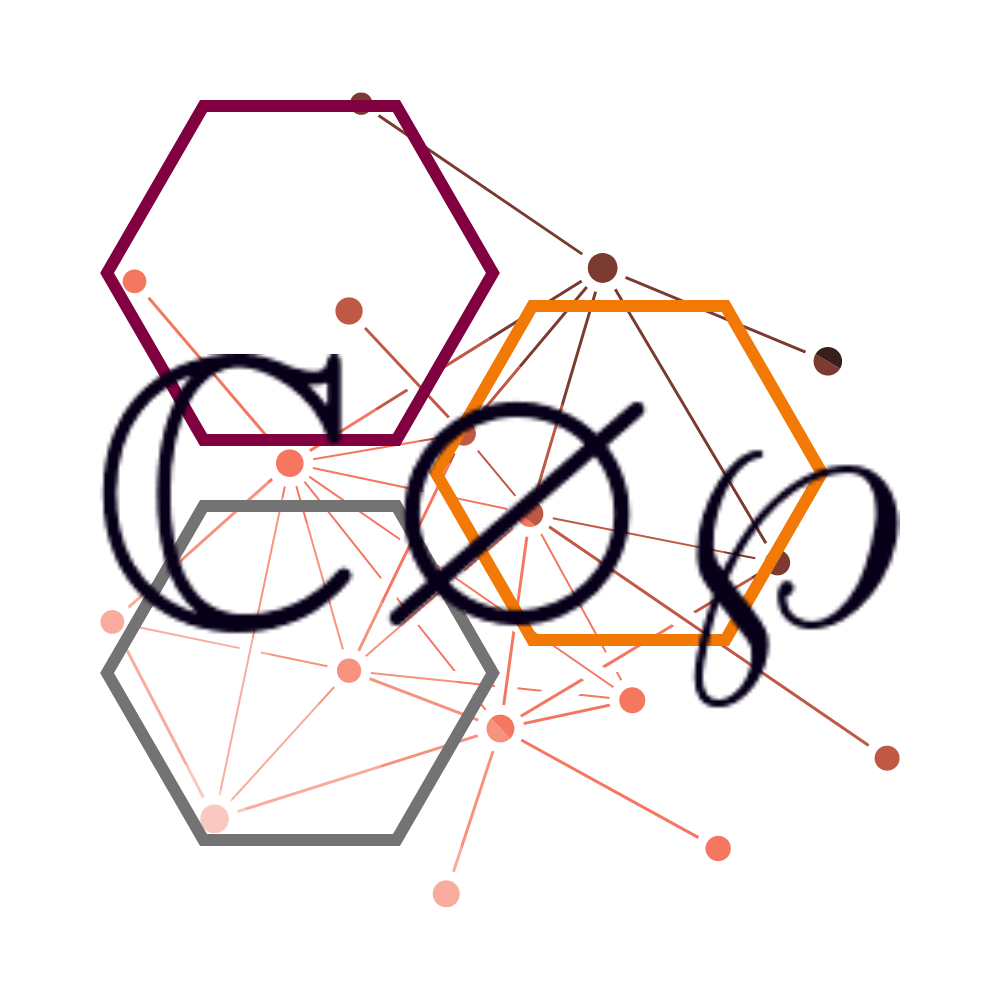
\includegraphics[width=10cm]{img/Logo COP SE.png}
                }
            }
        \end{center}
    }
}
    \newpage
    \maketitle
    \newpage
    \begin{lstlisting}[language=python, caption=Función dibuja\_matriz()]
def dibuja_matriz(M):
    for i in range(len(M)):
        print('[', end='')
        for j in range(len(M[i])):
            print('{:^3n}'.format(M[i][j]), end='')
        print(']')
\end{lstlisting}
    \section{Eliminación de bucles (loops)}
La función \texttt{\textbf{elimina\_bucles(M)}} recorre una matriz \texttt{\textbf{M}} y le asigna el valor $0$ a las entradas \texttt{\textbf{m$_{i,i}$}}, entradas que representan bucles de longitud uno.
\begin{lstlisting}[language=python, caption=Función elimina\_bucles(M)]
def elimina_bucles(M):
    n = len(M)
    for i in range(n):
        M[i][i] = 0
\end{lstlisting}
    \section{Vértices}
La función \texttt{\textbf{crea\_vértices(M)}} recorre una matriz \texttt{\textbf{M}}, lista los vértices adyacentes y convierte las entradas \texttt{\textbf{m$_{i,j}$}} en un diccionario que contiene el número de vértice, vértices adyacentes y un estado que indica si está conectado o no, para listarlas y devolver la lista de los vértices.
\begin{lstlisting}[language=python, caption=Función crea\_vértices(M)]
def crea_vertices(M):
    n = len(M)
    vertices = []
    vecinos = []
    vecinos_vj = []
    for i in range(n):
        for j in range(n):
            if M[i][j] != 0:
                vecinos_vj.append(j + 1)
        vecinos.append(dict([("vecinos", vecinos_vj.copy())]))
        vecinos_vj.clear()
    for i in range(n):
        vertices.append(dict([("vertice", i + 1), ("vecinos", vecinos[i]), ("conectado", False)]))
    return vertices
\end{lstlisting}
    \section{Entrada}
La función \texttt{\textbf{lee\_matriz(M)}} solicita el número de vértices del grafo, lee una matriz triangular inferior ($n\times n$), es decir las entradas \texttt{\textbf{m$_{i,j}$ con $i\ge j$}}, donde las  entradas \texttt{\textbf{m$_{i,j}$ con $i=j$}} deben ser pares, pues la diagonal representa a los bucles (loops), y luego le asigna el valor de las entradas \texttt{\textbf{m$_{i,j}$}} a las entradas \texttt{\textbf{m$_{j,i}$}}, para asegurar que sea una matriz de adyacencia (debe ser simétrica). Retorna la matriz generada.
\begin{lstlisting}[language=python, caption=Función lee\_matriz()]
def lee_matriz():
    n = int(input("Ingrese el numero de vertices del grafo: "))
    M = [[-1] * n for i in range(n)]
    for i in range(n):
        for j in range(i + 1):
            if i == j:
                M[i][j] = valida_entrada(i, j, True)
            else:
                M[i][j] = valida_entrada(i, j, False)
            if i > j:
                M[j][i] = M[i][j]
    return M
\end{lstlisting}
\subsection{Validación}
La función \texttt{\textbf{valida\_entrada(M)}} valida que los valores leídos sean numéricos y que las entradas de la diagonal sean números pares.
\begin{lstlisting}[language=python, caption=Función valida\_entrada()]
def valida_bucles(i, j, flag: bool) -> int:
    resul: int = 1
    if flag:
        while resul % 2 != 0:
            while True:
                try:
                    resul = int(input(
                        "Ingrese la entrada M[{0}][{1}] (Esta debe ser par): ".format(str(i + 1), str(j + 1))))
                    break
                except:
                    print("No es un valor valido!")
        return resul
    else:
        while True:
            try:
                resul = int(input("Ingrese la entrada M[{0}][{1}]: ".format(str(i + 1), str(j + 1))))
                return resul
            except:
                print("No es un valor valido!")
\end{lstlisting}
    \section{Busqueda en anchura}
La función \texttt{\textbf{generar\_arbol\_anchura(M)}} genera una matriz de adyacencia de un árbol generador dada una matriz \texttt{\textbf{M}}, a partir del algoritmo de busqueda por anchura.
Esta función, al igual que la de entrada, genera una matriz triangular inferior recorriendo los vértices, conectando con sus vecinos (cambiando su estado) y posteriormente completa la matriz simétrica, retornando esta última.
\begin{lstlisting}[language=python, caption=Función generar\_arbol\_anchura(M)]
def generar_arbol_anchura(M):
    n = len(M)
    arbol_MA = [[0] * n for i in range(n)]
    vertices = crea_vertices(M)
    for i in range(n):
        for j in vertices[i].get("vecinos").values():
            for k in j:
                if not vertices[k - 1].get("conectado"):
                    if k - 1 >= i:
                        arbol_MA[i][k - 1] += 1
                        if k - 1 > i:
                            arbol_MA[k - 1][i] = arbol_MA[i][k - 1]
                    auctualizacion_estado = {"conectado": True}
                    vertices[k - 1].update(auctualizacion_estado)
    return arbol_MA
\end{lstlisting}
    \section{Busqueda en profundidad}
La función \texttt{\textbf{generar\_arbol\_profundidad(M)}} genera una matriz de adyacencia de un árbol generador dada una matriz \texttt{\textbf{M}}, a partir del algoritmo de busqueda por profundidad.
Esta función,  hace uso de una pila auxiliar para conectar un vértice adyacente al anterior.
\begin{lstlisting}[language=python, caption=Función generar\_arbol\_profundidad(M)]
    def generar_arbol_profundidad(M):
        V = set()  # Conjunto de vertices ya conectados
        Vaux = set()  # Conjunto de vertices auxiliar
        vecino = 0  # Vecino mas pequeno
        Pila = []  # Pila auxiliar
        n = len(M)  # Numero de vertices
        MA = [[0 for i in range(n)] for i in range(n)]  # Matriz de adyacencia
        vertices = crea_vertices(M)
        Pila.append(1)
        V.add(1)
        while len(Pila) != 0:  # Acaba cuando la pila esta vacia
            u = Pila[-1]  # Tomamos el ultimo elemento de la pila
            Vaux = set(vertices[u - 1].get("vecinos"))  # Obtenemos el conjunto de vertices no conectados a u
            if len(Vaux - V) > 0:  # Si hay al menos un vecino no conectado a u
                vecino = min(Vaux - V)  # Tomamos el vertice no conectado mas pequeno
                MA[u - 1][vecino - 1] = 1  # Los conectamos
                MA[vecino - 1][u - 1] = 1
                if vecino not in Pila:  # Si el vecino no estaba en la pila, lo agregamos
                    Pila.append(vecino)
                V.add(vecino)  # Agregamos al vecino al conjunto de vertices ya conectados
            else:
                Pila.remove(u)  # Si u no tiene vecinos sin conectar, lo quitamos de la pila
        Pila.clear()
        V.clear()
        Vaux.clear()
        return MA
\end{lstlisting}
\end{document}